\documentclass[a4paper, 14pt]{extarticle}

% Поля
%--------------------------------------
\usepackage{geometry}
\geometry{a4paper,tmargin=2cm,bmargin=2cm,lmargin=3cm,rmargin=1cm}
%--------------------------------------


%Russian-specific packages
%--------------------------------------
\usepackage[T2A]{fontenc}
\usepackage[utf8]{inputenc} 
\usepackage[english, main=russian]{babel}
%--------------------------------------

\usepackage{textcomp}

% Красная строка
%--------------------------------------
\usepackage{indentfirst}               
%--------------------------------------             


%Graphics
%--------------------------------------
\usepackage{graphicx}
\graphicspath{ {./images/} }
\usepackage{wrapfig}
%--------------------------------------

% Полуторный интервал
%--------------------------------------
\linespread{1.3}                    
%--------------------------------------

%Выравнивание и переносы
%--------------------------------------
% Избавляемся от переполнений
\sloppy
% Запрещаем разрыв страницы после первой строки абзаца
\clubpenalty=10000
% Запрещаем разрыв страницы после последней строки абзаца
\widowpenalty=10000
%--------------------------------------

%Списки
\usepackage{enumitem}

%Подписи
\usepackage{caption} 

%Гиперссылки
\usepackage{hyperref}

\hypersetup {
	unicode=true
}

%Рисунки
%--------------------------------------
\DeclareCaptionLabelSeparator*{emdash}{~--- }
\captionsetup[figure]{labelsep=emdash,font=onehalfspacing,position=bottom}
%--------------------------------------

\usepackage{tempora}

%Листинги
%--------------------------------------
\usepackage{listings}
\lstset{
  basicstyle=\ttfamily\footnotesize, 
  %basicstyle=\footnotesize\AnkaCoder,        % the size of the fonts that are used for the code
  breakatwhitespace=false,         % sets if automatic breaks shoulbd only happen at whitespace
  breaklines=true,                 % sets automatic line breaking
  captionpos=t,                    % sets the caption-position to bottom
  inputencoding=utf8,
  frame=single,                    % adds a frame around the code
  keepspaces=true,                 % keeps spaces in text, useful for keeping indentation of code (possibly needs columns=flexible)
  keywordstyle=\bf,       % keyword style
  numbers=left,                    % where to put the line-numbers; possible values are (none, left, right)
  numbersep=5pt,                   % how far the line-numbers are from the code
  xleftmargin=25pt,
  xrightmargin=25pt,
  showspaces=false,                % show spaces everywhere adding particular underscores; it overrides 'showstringspaces'
  showstringspaces=false,          % underline spaces within strings only
  showtabs=false,                  % show tabs within strings adding particular underscores
  stepnumber=1,                    % the step between two line-numbers. If it's 1, each line will be numbered
  tabsize=2,                       % sets default tabsize to 8 spaces
  title=\lstname                   % show the filename of files included with \lstinputlisting; also try caption instead of title
}
%--------------------------------------

%%% Математические пакеты %%%
%--------------------------------------
\usepackage{amsthm,amsfonts,amsmath,amssymb,amscd}  % Математические дополнения от AMS
\usepackage{mathtools}                              % Добавляет окружение multlined
\usepackage[perpage]{footmisc}
%--------------------------------------

%--------------------------------------
%			НАЧАЛО ДОКУМЕНТА
%--------------------------------------

\begin{document}

%--------------------------------------
%			ТИТУЛЬНЫЙ ЛИСТ
%--------------------------------------
\begin{titlepage}
\thispagestyle{empty}
\newpage


%Шапка титульного листа
%--------------------------------------
\vspace*{-60pt}
\hspace{-65pt}
\begin{minipage}{0.3\textwidth}
\hspace*{-20pt}\centering

\includegraphics[width=\textwidth]{emblem}
\end{minipage}
\begin{minipage}{0.67\textwidth}\small \textbf{
\vspace*{-0.7ex}
\hspace*{-6pt}\centerline{Министерство науки и высшего образования Российской Федерации}
\vspace*{-0.7ex}
\centerline{Федеральное государственное бюджетное образовательное учреждение }
\vspace*{-0.7ex}
\centerline{высшего образования}
\vspace*{-0.7ex}
\centerline{<<Московский государственный технический университет}
\vspace*{-0.7ex}
\centerline{имени Н.Э. Баумана}
\vspace*{-0.7ex}
\centerline{(национальный исследовательский университет)>>}
\vspace*{-0.7ex}
\centerline{(МГТУ им. Н.Э. Баумана)}}
\end{minipage}
%--------------------------------------

%Полосы
%--------------------------------------
\vspace{-25pt}
\hspace{-35pt}\rule{\textwidth}{2.3pt}

\vspace*{-20.3pt}
\hspace{-35pt}\rule{\textwidth}{0.4pt}
%--------------------------------------

\vspace{1.5ex}
\hspace{-35pt} \noindent \small ФАКУЛЬТЕТ\hspace{80pt} <<Информатика и системы управления>>

\vspace*{-16pt}
\hspace{47pt}\rule{0.83\textwidth}{0.4pt}

\vspace{0.5ex}
\hspace{-35pt} \noindent \small КАФЕДРА\hspace{50pt} <<Теоретическая информатика и компьютерные технологии>>

\vspace*{-16pt}
\hspace{30pt}\rule{0.866\textwidth}{0.4pt}
  
\vspace{11em}

\begin{center}
\Large {\bf Лабораторная работа № 2} \\
\large {\bf по курсу <<Разработка мобильных приложений>>} \\
\large <<Реализация приложения на основе виджета>>
\end{center}\normalsize

\vspace{8em}


\begin{flushright}
  {Студентка группы ИУ9-72Б Самохвалова П. С. \hspace*{15pt}\\
  \vspace{2ex}
  Преподаватель Посевин Д. П.\hspace*{15pt}}
\end{flushright}

\bigskip

\vfill
 

\begin{center}
\textsl{Москва 2023}
\end{center}
\end{titlepage}
%--------------------------------------
%		КОНЕЦ ТИТУЛЬНОГО ЛИСТА
%--------------------------------------

\renewcommand{\ttdefault}{pcr}

\setlength{\tabcolsep}{3pt}
\newpage
\setcounter{page}{2}

\section{Задание}\label{Sect::task}

Вариант 15.

Используя 26 виджет реализовать программу отправки электронных сообщений пользователям из списка, текст сообщения и тема сообщения вводятся из отдельных полей. Пользователь приложения вводит только имя или фамилию получателя, адрес электронной почты он видеть не должен.

\section{Практическая реализация}\label{Sect::code}

Исходный код программы представлен в листинге~\ref{lst:code1}.

\begin{lstlisting}[language={},caption={Отправка электронных сообщений},label={lst:code1}]
import 'dart:async';
import 'dart:io';

import 'package:flutter/material.dart';
import 'package:flutter_email_sender/flutter_email_sender.dart';
import 'package:image_picker/image_picker.dart';
import 'package:path_provider/path_provider.dart';

void main() => runApp(MyApp());


class MyApp extends StatelessWidget {
  @override
  Widget build(BuildContext context) {
    return MaterialApp(
      theme: ThemeData(primaryColor: Colors.red),
      home: EmailSender(),
    );
  }
}

class EmailSender extends StatefulWidget {
  const EmailSender({Key? key}) : super(key: key);

  @override
  _EmailSenderState createState() => _EmailSenderState();
}

class _EmailSenderState extends State<EmailSender> {
  List<String> attachments = [];
  bool isHTML = false;

  final _nameController = TextEditingController(text: 'Receiver name');
  final _recipientController = TextEditingController(text: 'example@example.com');
  final _subjectController = TextEditingController(text: 'The subject');
  final _bodyController = TextEditingController(text: 'Mail body.');

  List<String> names = ['Polina', 'Dmitry', 'Name 3', 'Name 4', 'Name 5'];
  String? selectedItem = 'Polina';

  Future<void> send() async {

    if (selectedItem == "Polina") {
      _recipientController.text = "sam53351@yandex.ru";
      _nameController.text = "Polina";
    } else if (selectedItem == "Dmitry") {
      _recipientController.text = "dmitry@yandex.ru";
      _nameController.text = "Dmitry";
    }

    final Email email = Email(

      body: _bodyController.text,
      subject: _subjectController.text,
      recipients: [_recipientController.text],
      attachmentPaths: attachments,
      isHTML: isHTML,
    );

    String platformResponse;

    try {
      await FlutterEmailSender.send(email);
      platformResponse = 'success';
    } catch (error) {
      print(error);
      platformResponse = error.toString();
    }

    if (!mounted) return;

    ScaffoldMessenger.of(context).showSnackBar(
      SnackBar(
        content: Text(platformResponse),
      ),
    );
  }

  @override
  Widget build(BuildContext context) {
    return Scaffold(
      appBar: AppBar(
        title: Text('Plugin example app'),
        actions: <Widget>[
          IconButton(
            onPressed: send,
            icon: Icon(Icons.send),
          )
        ],
      ),
      body: Padding(
        padding: EdgeInsets.all(8.0),
        child: Column(
          mainAxisSize: MainAxisSize.max,
          // mainAxisAlignment: MainAxisAlignment.spaceBetween,
          crossAxisAlignment: CrossAxisAlignment.center,
          children: <Widget>[

            DropdownButton <String> (
              value: selectedItem,
              items: names
                  .map((name) => DropdownMenuItem<String>(
                value: name,
                child: Text(name, style: TextStyle(fontSize: 24)),
              ))
                  .toList(),
              onChanged: (name) => setState(() => selectedItem = name!),

            ),

            Padding(
              padding: EdgeInsets.all(8.0),
              child: TextField(
                controller: _subjectController,
                decoration: InputDecoration(
                  border: OutlineInputBorder(),
                  labelText: 'Subject',
                ),
              ),
            ),

            Expanded(
              child: Padding(
                padding: EdgeInsets.all(8.0),
                child: TextField(
                  controller: _bodyController,
                  maxLines: null,
                  expands: true,
                  textAlignVertical: TextAlignVertical.top,
                  decoration: InputDecoration(
                      labelText: 'Body', border: OutlineInputBorder()),
                ),
              ),
            ),
            CheckboxListTile(
              contentPadding:
              EdgeInsets.symmetric(vertical: 0.0, horizontal: 8.0),
              title: Text('HTML'),
              onChanged: (bool? value) {
                if (value != null) {
                  setState(() {
                    isHTML = value;
                  });
                }
              },
              value: isHTML,
            ),

            Padding(
              padding: EdgeInsets.all(8.0),
              child: Column(
                children: <Widget>[
                  for (var i = 0; i < attachments.length; i++)
                    Row(
                      children: <Widget>[
                        Expanded(
                          child: Text(
                            attachments[i],
                            softWrap: false,
                            overflow: TextOverflow.fade,
                          ),
                        ),
                        IconButton(
                          icon: Icon(Icons.remove_circle),
                          onPressed: () => {_removeAttachment(i)},
                        )
                      ],
                    ),
                  Align(
                    alignment: Alignment.centerRight,
                    child: IconButton(
                      icon: Icon(Icons.attach_file),
                      onPressed: _openImagePicker,
                    ),
                  ),
                  TextButton(
                    child: Text('Attach file in app documents directory'),
                    onPressed: () => _attachFileFromAppDocumentsDirectoy(),
                  ),
                ],
              ),
            ),
          ],
        ),
      ),
    );
  }

  void _openImagePicker() async {
    final picker = ImagePicker();
    XFile? pick = await picker.pickImage(source: ImageSource.gallery);
    if (pick != null) {
      setState(() {
        attachments.add(pick.path);
      });
    }
  }

  void _removeAttachment(int index) {
    setState(() {
      attachments.removeAt(index);
    });
  }

  Future<void> _attachFileFromAppDocumentsDirectoy() async {
    try {
      final appDocumentDir = await getApplicationDocumentsDirectory();
      final filePath = appDocumentDir.path + '/file.txt';
      final file = File(filePath);
      await file.writeAsString('Text file in app directory');

      setState(() {
        attachments.add(filePath);
      });
    } catch (e) {
      ScaffoldMessenger.of(context).showSnackBar(
        SnackBar(
          content: Text('Failed to create file in applicion directory'),
        ),
      );
    }
  }
}
\end{lstlisting}

\section{Результаты}\label{Sect::res}

Результаты работы программы представлены на рисунках~\ref{fig:img1}~--~\ref{fig:img4}.

\begin{figure}[!htb]
	\centering
	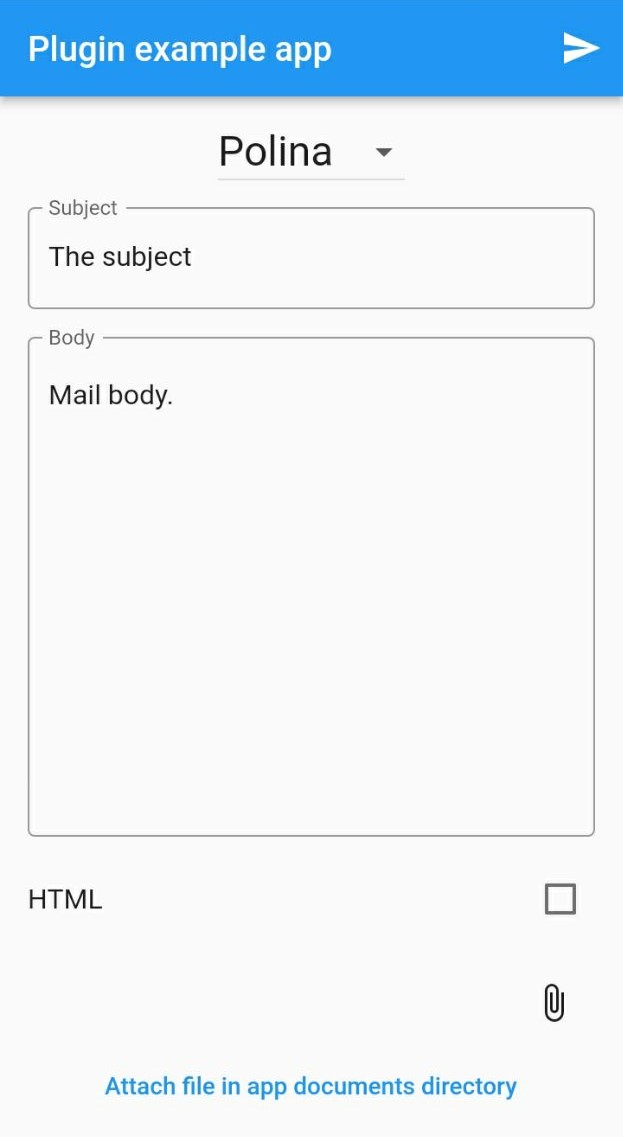
\includegraphics[width=0.8\textwidth]{img1}
\caption{Форма ввода электронного сообщения}
\label{fig:img1}
\end{figure}

\begin{figure}[!htb]
	\centering
	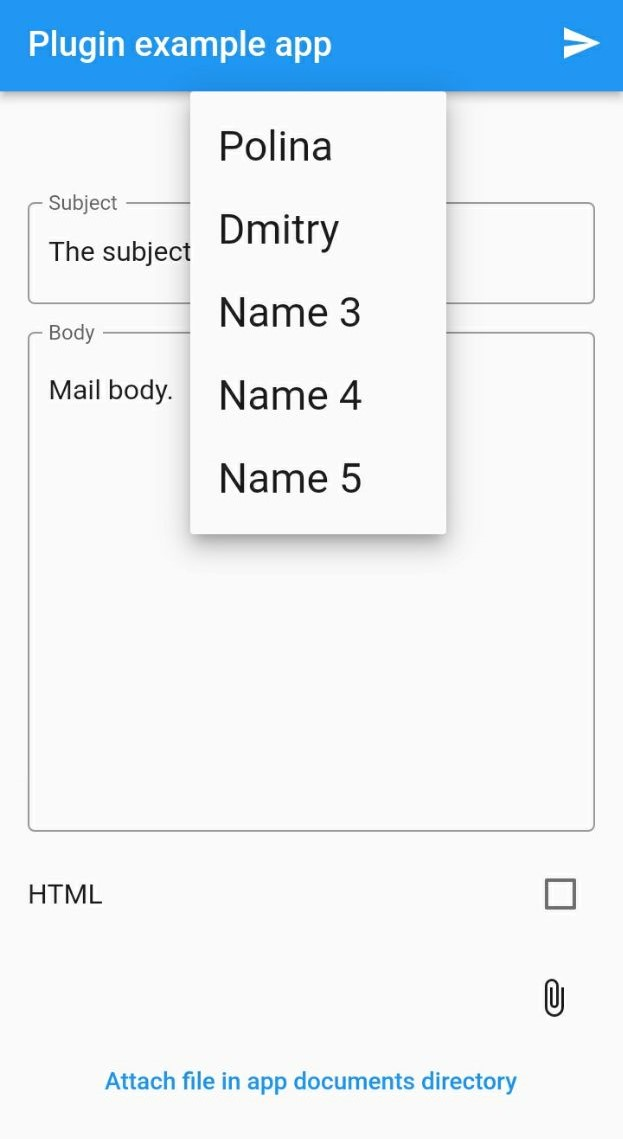
\includegraphics[width=0.8\textwidth]{img2}
\caption{Выбор пользователя из списка}
\label{fig:img2}
\end{figure}

\begin{figure}[!htb]
	\centering
	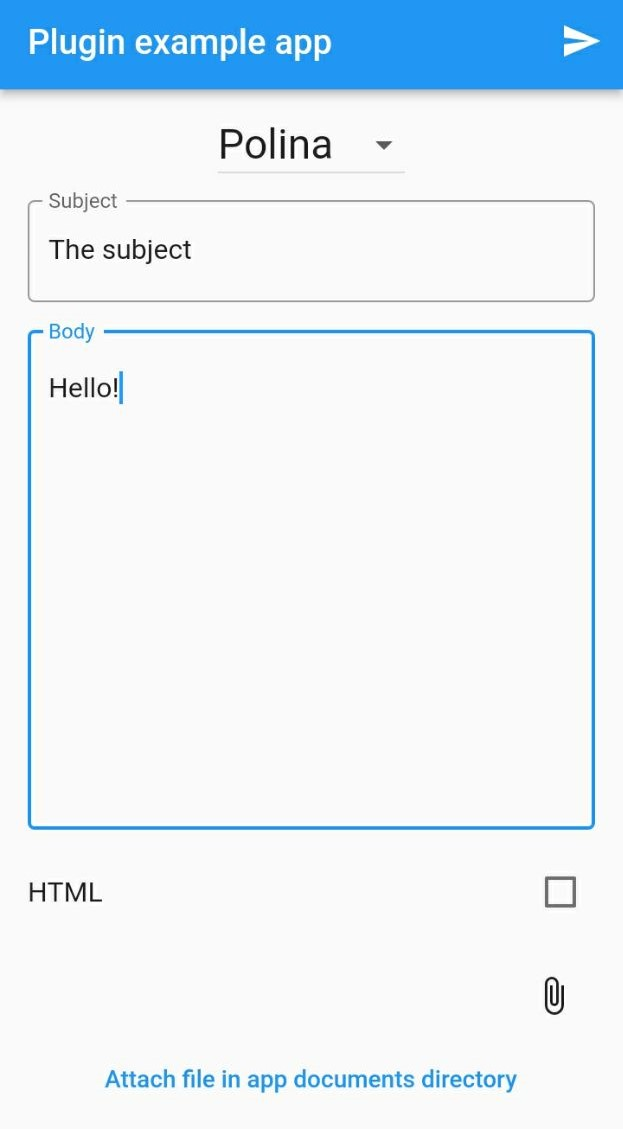
\includegraphics[width=0.8\textwidth]{img3}
\caption{Ввод текста письма}
\label{fig:img3}
\end{figure}

\begin{figure}[!htb]
	\centering
	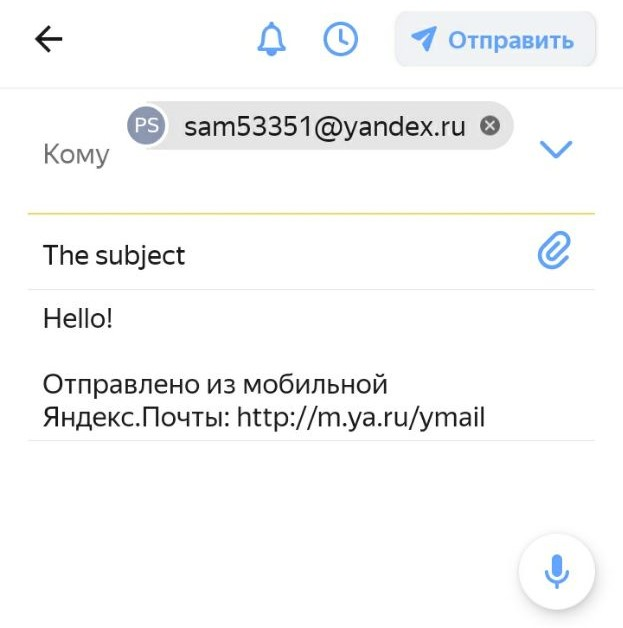
\includegraphics[width=0.8\textwidth]{img4}
\caption{Отправка письма}
\label{fig:img4}
\end{figure}

\section{Выводы}\label{Sect::conclusion}

В результате выполнения лабораторной работы была реализована программа отправки электронных сообщений пользователям из списка.

\end{document}
